\documentclass[12pt]{article}

\usepackage{sbc-template}

\usepackage{graphicx,url}

%\usepackage[brazil]{babel}   
\usepackage[utf8]{inputenc}  

     
\sloppy

\title{Relatório Intermediario Pocket Mips\\ Laboratório de Hardware}

\author{Diogo Oliveira Roman\inst{1}, Rodrigo Gonsalvez de branco\inst{1}}


\address{Faculdade de Computação -- Universidade Federal do Mato Grosso do Sul
  (UFMS)\\
  %Caixa Postal 15.064 -- 91.501-970 -- Porto Alegre -- RS -- Brazil
%\nextinstitute
%  Department of Computer Science -- University of Durham\\
%  Durham, U.K.
%\nextinstitute
%  Departamento de Sistemas e Computa��o\\
%  Universidade Regional de Blumenal (FURB) -- Blumenau, SC -- Brazil
  \email{\{diogo.or,rodrigo.g.branco\}@gmail.com}
}

\begin{document} 

\maketitle


\section{Informações Gerais}

\textbf{Grupo:} Diogo Oliveira Roman, Rodrigo Gonsalvez de Branco.

Utilizamos o sistema Ghdl para fazer a compilação e o editor gedit no sistema operacional Linux. Além disso estamos usando svn para controle de versão.

\section{Modulo Implementados} \label{sec:modulos}

Todos os módulos já foram implementados. Abaixo descreveremos a implementação.

\subsection{Gerador de Clock}

A arquitetura foi implementada com dois processos, um processo é encarregado de gerar o clock com uma frequencia de 2 ns, este utiliza um sinal auxiliar da arquitetura identificado como \textit{clock}, dessa maneira o clock ainda não é propagado para fora do circuito. Um detalhe desse processo é que ele só fará a modificação no sinal \textit{clock}, caso o sinal \textit{canHalt} for igual a zero, dessa maneira é possível interromper a geração de clock, atribuindo '1' a \textit{canHalt}.

O outro processo é encarregado por modificar o sinal da arquitetura \textit{canHalt} e o sinal do circuito \textit{Clk}. Além disso sua lista de sensibilidade é composta pelos sinais \textit{clock} e \textit{Halt}, onde o primeiro é interno à arquitetura e outro pertence ao circuito. Caso as condições sejam satisfeitas o sinal de \textit{clock} é atribuito para \textit{Clk} e assim é propagado para fora do circuito, pois \textit{Clk} é o sinal de saída. Além disso caso o sinal do circuito \textit{Halt} sofrer um evento e mudar para '1' deve-se interromper a geração de clock, como mencionado anteriormente isso pode ser feito atribuindo o valor '1' à variável \textit{canHalt}.

\subsection{Registrador PC}

Esta arquitetura é composta por um único processo sincronizado pelo clock, sempre que o clock esta na borda de subida o valor do sinal \textit{NewPC} é atribuído ao \textit{CurrentPC}, mesmo quando o valor não muda esta atribuição deve acontecer, pois isso garante o funcionamento dessa entidade como um registrador.

\subsection{Somador de 1 Bit}

Esta arquitetura é totalmente estrutural, ou seja sem processo, ela simplesmente implementa o circuito somador de 1 bit. Como esse circuito é bem conhecido não entraremos nos detalhes de sua implementação neste trabalho, visto que a forma estrutural traduz exatamente o circuito para a linguagem VHDL, dessa maneira nenhum detalhe de implementação diferente do circuito foi necessário.

\subsection{Somador Completo}

Esta arquitetura é totalmente estrutural, e consiste simplesmente da ligação entre os somadores de 1 bit. A posições dos vetores de bits \textit{A}, \textit{B} e \textit{Sum} correspondem aos sinais \textit{A}, \textit{B} e \textit{Sum} em cada somador de 1 bit. Ja as posições do também vetor de bits \textit{carry} correspondem ao sinal \textit{carryIn} e \textit{carryOut} de cada somador de 1 bit.

A implementa desse somador foi feita seguindo o padrão ja conhecido na literatura, portando não entraremos em detalhes. A única observação a ser feita é que a ligação entre o \textit{carryOut} e o \textit{carryIn} de somadores de 1 bit respectivos é feita através do vetor de bits \textit{carry} dessa arquitetura. Cada posição desse vetor corresponde ao \textit{carryOut} dos somadores de 1 bit na respectiva posição, ou seja, o somador de 1 bit para os bits da posição 5 dos operandos armazenam o \textit{carryOut} também na posição 5 do vetor \textit{carry}, dessa maneira basta atribuir ao \textit{carryIn} a posição anterior no vetor \textit{carry} para fazer a ligação entre o \textit{carryIn} do somador atual com o \textit{carryOut} do somador anterior.

\subsection{Unidade Logico Aritimetica}

A implementação dessa arquitetura é simplesmente a instanciação de um somador completo e a manipulação dos seus operandos B e carryIn. Esta manipulação se deu da seguinte maneira:
\begin{enumerate}
 \item Caso seja soma: Atribui os operandos da ALU para o somador sem nenhuma alteração.
 \item Caso seja subtração: Nega bit a bit o operando \textit{B} e atribui um para o \textit{carryIn} da ALU.
\end{enumerate}

\subsection{Memória de Dados}

Implementamos a memória de dados utilizando um único processo, onde na primeira parte foi calculado o endereço a ser acessado na memória, isso nada mais é que a conversão do sinal \textit{Address} de binário para decimal. Isso foi necessário para acessar o índice do vetor bi-dimensional \textit{Memory}, que justamente é a representação da memória.

A leitura da memória é feita em qualquer momento, independente do clock, já a escrita é feita apenas na borda de subida.

\subsection{Memória de Instruções}

Esta memória poderia ser exatamente uma copia da memória de dados, contudo para isso deveríamos fazer outra entidade para carregar as instruções do arquivo para ela. Pela simplicidade preferimos fazer o carregamento das instruções dentro dessa entidade mesmo.

Dessa forma foi feito dois processos, um faz apenas a leitura da memória de acordo com o sinal de entrada \textit{ReadAddress} e retorna a instrução pela variável \textit{Instruction}.

Já o outro processo controla o carregamento da memória, ele deve carregar todas as instruções do arquivo especificado na entrada padrão para a memória de instruções antes de começar a execução do processador como um todo. 
Dessa maneira inserimos dois sinais de controle, para que fosse possível iniciar o processamento assim que a memória de instruções estivesse totalmente carregada, isso foi preciso pois como não sabemos a quantidade de instruções que serão carregada não podemos prever quantos ciclos de clock o este carregamento pode levar. Isso pode causar o incremento do PC antes da hora, pois este esta sincronizado apenas com o clock. Portando enquanto carregamos a memória o gerador de clock está parado.

\subsection{Banco de Registradores}

Um problema que encontramos ao implementar o banco de registradores foi como definir qual registrador acumulador o dados deverá ser escrito ou lido. Para soluciona-lo inserimos dois sinais de controle identificados como \textit{WriteHidden} e \textit{WhichHidden}, onde o primeiro indica se deverá ser feita uma escrita em algum acumulador e o segundo em qual acumulador essa escrita será feita, caso seja 1 o acumulador BC deve ser carregado, caso contrário o AC que deverá receber o valor. Além dessas variáveis de controle inserimos um vetor de bits para retornar qual o valor lido nos acumuladores, a esse vetor demos a identificação de \textit{ReadHidden}.

\subsection{Extensor de sinal}

Esta entidade é bem simples, de forma que foi trivial faze-la. Fizemos com um processo que apenas copia os dados de um vetor de 5 bits para outro de 8 bits, os 5 bits de mais baixa ordem do vetor menor vão para as cinco posições iguais no vetor maior, os bits que sobram são preenchidos com o bit de sinal, ou seja, da posição 5 até à 7 recebe a posição 4 do vetor menor.

\subsection{Unidade de Controle}

Apesar do código extenso dessa entidade, ela não oferece muitas dificuldades. Nela fazemos controle de todo o processador. Antes de qualquer ação uma verificação na condição da memoria de instruções é feita, ou seja, verifica se esta já esta totalmente carregada, e caso afirmativo o processamento da unidade de controle continua e faz uma séride de atribuições aos diversos sinais de controle. Estas atribuições dependem apenas dos sinais de entrada \textit{aluOperation} e \textit{Func}, onde o primeiro é o código da operação que se deve executar e o segundo é usado apenas nas operações MTA, MFA, MTB, MFB.

Fazemos o controle da memória de instruções aqui através de num sinal de inicio de clock, ou seja, enquanto não for recebido o sinal de que a memória de instruções esta carregada a geração de clock não inicia.

\subsection{Caminho de Dados}

Esta entidade é o caminho de dados, nela fazemos a ligação entre todas as outras entidades citadas e ainda entre circuitos primitivo como portas and e multiplexadores. Foi necessário a instanciação de vários sinais para fazer a ligação entre as entidades. Além disso incluímos outro processo que intercepta o sinal retornado pela memória de instruções e retorna na saída padrão a informação das instruções lida em ascii.

\section{Experimentos e Resultados}
Programa teste:
\begin{enumerate}
  \item ADDI 6
  \item MFA r1
  \item ADDI 4
  \item ADD r1
  \item SUB r1
  \item HALT
\end{enumerate}
Este programa faz o seguinte:
\begin{enumerate}
  \item AC = AC + 6
  \item r1 = AC + 0
  \item AC = AC + 4
  \item AC = AC + r1
  \item AC = AC - r1
  \item Interrompe o processo
\end{enumerate}
No fim o registrador AC deve armazenar o valor 10.
Isto pode ser visto na imagem de ondas abaixo.
\begin{figure}[ht]
\centering
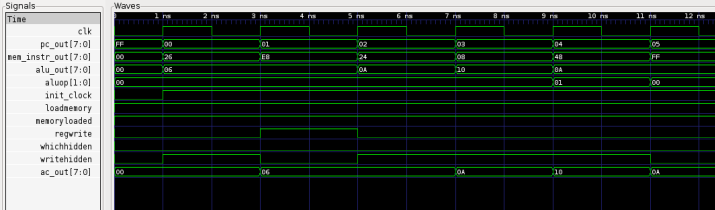
\includegraphics[width=1\textwidth]{onda.png}
\caption{Ondas geradas na execução do programa}
\label{fig:Arquivo de Ondas}
\end{figure}

No primeiro ciclo de clock a memória de instruções é carregada, porem isso foi feito muito rápido de maneira que foi imperceptível, nesse mesmo ciclo o PC é iniciado em 0 e a unidade de controle faz a leitura da primeira instrução, e ajusta os sinais de controle, é possível ver isso através da variável \textit{writehidden}.
Na borda de subida do segundo ciclo de clock o valor 6 é atribuído ao acumulador AC, o PC é incrementado e dessa maneira a instrução MFA é carregada, note que o sinal \textit{writehidden} volta ao valor 0, isto indica que a instrução recem carregada não escreverá nos acumuladores.
O processamento continúa de maneira analoga até o fim do programa. A variável \textit{ac\_out} armazena o valor do acumulador AC, dessa maneira
 pode-se visualizar a corretude do processador nesse teste.

\section{Conclusões}

O trabalho foi desenvolvido no tempo programado, agora a próxima etapa é otimizar o código e deixa-lo mais genérico quanto ao tamanho da memória, usando para isso o comando generic. Além disso falta testa-lo na FPGA, o que acreditamos que vai dar muitos problemas e provocar muitas mudanças no código.

As principais dificuldades encontradas foram questões praticas de simulação. Em alguns momentos perdemos muito tempo para descobrir alguns erros pois estávamos pensando no sistema como qualquer outro programa que estamos acostumado a fazer, principalmente no fato de termos que reatribuir valores a variáveis mesmo quando esses valore não mudam, algo desnecessário na programação comum.


%\section{References}

%\bibliographystyle{sbc}
%\bibliography{sbc-template}

\end{document}
